\documentclass[letterpaper,10pt,conference]{ieeeconf}
\IEEEoverridecommandlockouts
\overrideIEEEmargins
\usepackage{amsmath,amssymb,booktabs,multirow,array,tabularx,xcolor,url,graphicx}
\usepackage[colorlinks=true,urlcolor=blue,linkcolor=black,citecolor=black]{hyperref}
\def\UrlBreaks{\do\/\do\_\do\.\do\-}
\newcommand{\hfrepo}{\url{https://huggingface.co/mdhamidhosen/tartanimu-unified-hosen42}}
\newcommand{\ghrepo}{\url{https://github.com/hamidhosen42/TartanIMU-Challenge-Multi-Platform-Inertial-Odometry}}

\title{\LARGE \bf One Model, Four Bodies: Trajectory-Context Inertial Velocity Estimation\\
Across Cars, Quadrupeds, Drones and Handheld Sensors}

\author{Md.\ Hamid Hosen$^{1}$, Esfer Sami$^{1}$, Kahakashan Ashraf$^{1}$ and Foysal Emon Shanto$^{1}$%
\thanks{$^{1}$Team Hack2Publish. Affiliations to be added. Corresponding author: Md.\ Hamid Hosen,
{\tt\small mdhamidhosen4@gmail.com}}%
}

\begin{document}
\maketitle
\thispagestyle{empty}
\pagestyle{empty}

\begin{abstract}
Learned inertial odometry is usually trained and evaluated on one kind of platform at a time. We study the harder
setting posed by the TartanIMU Challenge at IROS 2026: a single network, with one set of weights, must predict the
body-frame velocity of a car, a quadruped robot, a racing drone and a handheld sensor from a 6-axis IMU alone,
without being told which platform it is looking at. We show that the decisive ingredient is context. Instead of
regressing each 1\,s window in isolation, our network reads 16\,s of a trajectory, predicts a dense velocity for the
whole span and averages overlapping predictions; this alone reduces the challenge score from about 0.30 to 0.22 on a
held-out split. Two further ingredients, a sampler that mirrors the per-platform and per-trajectory averaging of the
metric and augmentation that is exact under the sensor physics (random re-mounting applied to both signal and
label, gravity-aware time dilation), bring the held-out score to 0.198. The final 3.9\,M-parameter model, trained on
the challenge data only, reaches a TartanIMU Score of 0.219 on the 89-sequence test set (macro velocity error
0.18\,m/s), with 0.05--0.07\,m/s on car, quadruped and handheld data. We also analyse where the remaining error
lives: one drone source has an inverted gyroscope axis and an accelerometer that is not a rotation of its
ground-truth frame, and the racing-drone flights are recorded twice by two IMUs whose streams are offset from the
ground truth by different amounts, so that their labels disagree with each other by 0.15--0.9\,m/s. These
properties bound what any IMU-only model can achieve on that split. Code, weights and inference script are public.
\end{abstract}

\section{Introduction}
An inertial measurement unit is the one sensor that every mobile system carries. Estimating velocity from it alone is
attractive because it needs no line of sight, no lighting and no map, and difficult because the sensor measures
specific force and angular rate rather than motion: gravity, biases and the mounting of the sensor are folded into the
same six channels as the signal of interest, and integrating the signal amplifies every error. Learning-based
inertial odometry~\cite{ronin,tlio,ionet} has made this tractable for pedestrians and, more recently, for other
platforms~\cite{airio,tartanimu}, but nearly all of it is trained and evaluated one platform at a time.

The TartanIMU Challenge~\cite{tartanimu} asks a different question. Four embodiments -- a car, a quadruped, a racing
drone and a person carrying the sensor -- share one test set with no platform labels, and the entry must be a
single network with one set of weights. The score combines a per-window velocity error (AVE) with a 20\,m-segment
trajectory error (ATE$_{20}$), each averaged first over the windows of a trajectory, then over the trajectories of a
platform, then over the four platforms. This paper describes the entry of team Hack2Publish, which placed ninth on
the public leaderboard among 131 teams, and what we learned from building it.

Our starting observation was that the per-window velocity is far from independent across windows: the lag-1
autocorrelation is 0.85 for the car, 0.78 for the quadruped and 0.56 for the handheld sensor, and an oracle that
merely averages the true velocities of the two neighbouring windows halves the error of predicting zero. One second
of IMU is not enough to estimate gyroscope bias, low-frequency tilt or the embodiment; sixteen seconds is. Since the
test trajectories are provided whole, we built the entire solution around trajectory context. Our contributions are:
\begin{itemize}
    \item A trajectory-context architecture (conv stem, dilated temporal convolutions, small transformer, dense
    20\,Hz output with overlap averaging) that handles all four embodiments with no platform input, and a training
    recipe shaped after the challenge metric.
    \item A record of what did and did not help, with numbers, on a held-out split: context, schedule length and
    sampling helped every platform; strap-down features, a learned time-offset head, test-time augmentation and
    smoothing did not.
    \item An analysis of the drone data that explains most of the residual error and, we believe, bounds every
    IMU-only entry: an inverted gyroscope axis in one source, and inconsistent synchronisation and mounting between
    the two IMU recordings of each racing-drone flight.
\end{itemize}

\section{Related Work}
Classical strap-down inertial navigation integrates the IMU after removing gravity with an orientation estimate and
drifts within seconds without aiding~\cite{titterton}. Learned inertial odometry replaces the integration with a
regressor. RIDI~\cite{ridi} and IONet~\cite{ionet} regress pedestrian velocity or displacement from windows of IMU;
RoNIN~\cite{ronin} regresses velocity in a gravity-aligned frame with a ResNet, LSTM or TCN over 1--2\,s windows;
TLIO~\cite{tlio} regresses displacement with an uncertainty and fuses it in an EKF. AirIMU~\cite{airimu} and
AirIO~\cite{airio} extend learned inertial odometry to drones by learning the sensor noise model and by regressing in
the body frame, which is also the target frame of the challenge. Tartan IMU~\cite{tartanimu} is the first attempt at
a foundation model for inertial positioning across platforms and provides the challenge baseline: a shared ResNet-LSTM
trunk with per-platform heads. The challenge forbids per-platform routing, so our model has no heads at all; the
embodiment is inferred implicitly.

Two ideas we rely on have precedents. Using more context than the window being predicted is natural for sequence
models and is used by RoNIN's LSTM variant and by TLIO's filter; we take it further by predicting a whole 16\,s span
at once and averaging overlapping spans, which turned out to matter more than any architectural choice. Physically
exact augmentation of inertial data, in particular random rotations applied consistently to signal and label, is
standard in the pedestrian literature~\cite{ronin}; our time-dilation augmentation uses the gravity vector available
at training time to scale only the dynamic part of the acceleration.

\section{Method}
\subsection{Problem}
A trajectory is a sequence of 200\,Hz IMU samples $x_t = [a_t, \omega_t] \in \mathbb{R}^6$ with gravity retained.
Window $k$ is the 200 samples $x_{200k..200k+199}$, and the target is the mean body-frame velocity $v_k \in
\mathbb{R}^3$ over that window. The score is $0.6\,\mathrm{AVE}/0.7356 + 0.4\,\mathrm{ATE}_{20}/3.116$, where AVE is
the mean Euclidean error of $\hat v_k$ and ATE$_{20}$ integrates $\hat v_k$ (rotated with the ground-truth orientation,
which the model never sees) over 20\,m pieces of the true path and takes the RMS error after SE(3) alignment. Both
are macro-averaged over platforms and averaged per trajectory within a platform.

\subsection{Architecture}
Fig.~\ref{fig:pipeline} shows the network. The input is a chunk of $T=16$ consecutive windows, $3200 \times 6$ raw
samples, each channel divided by a fixed constant ($3\,\mathrm{m/s^2}$, $0.4\,\mathrm{rad/s}$) with no mean
subtraction, so that gravity stays available as a tilt cue and rotation augmentation stays exact. A two-layer strided
convolution (kernels 9 and 11, strides 2 and 5) produces 20\,Hz tokens of width 192. A parameter-free block computes
strap-down features on the same chunk: the gyroscope is integrated into a per-token relative orientation (a parallel
prefix product of rotation matrices), the accelerometer is rotated into the frame of the chunk start, its chunk mean
serves as a gravity estimate, and the de-gravitated acceleration and its integral are rotated back into the current
body frame; the features are computed for both signs of $\omega_z$ (Sec.~\ref{sec:data}) and added to the tokens
through a $1\times 1$ projection. Eight residual blocks of depthwise convolutions (kernel 5, dilations 1, 2, 4, 8, 16,
32, 1, 2) with pointwise MLPs and GroupNorm give a receptive field of about 13\,s; a three-layer pre-norm transformer
encoder (4 heads, learned positions) mixes the 320 tokens; a linear head outputs a velocity per token. The prediction
for window $k$ is the mean of its 20 tokens. An attention-pooled descriptor feeds a 4-way platform classifier that
exists only in the training graph. The model has 3.9\,M parameters.

\begin{figure}[t]
    \centering
    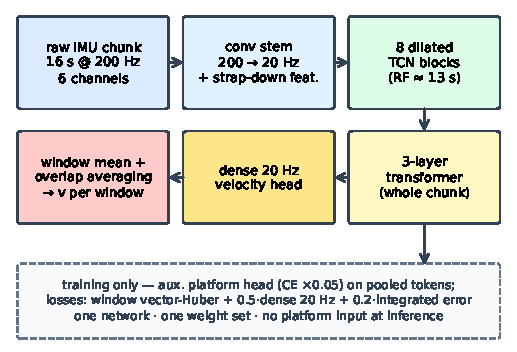
\includegraphics[width=\linewidth]{figures/pipeline.pdf}
    \caption{The network. One set of weights for all platforms; the platform head in the dashed box is a training
    signal only.}
    \label{fig:pipeline}
\end{figure}

\subsection{Losses and Sampling}
The loss is $L = L_{\mathrm{win}} + 0.5\,L_{\mathrm{dense}} + 0.2\,L_{\mathrm{drift}} + 0.05\,L_{\mathrm{plat}}$:
a Huber loss ($\beta = 0.25$\,m/s) on the norm of the per-window error, the same loss on the 20\,Hz output against
10-sample means of the ground-truth velocity, an integrated error
$L_{\mathrm{drift}} = \frac{1}{T}\sum_t \lVert \sum_{k \le t} (\hat v_k - v_k)\rVert / \sqrt{t}$ that penalises the
correlated bias which ATE$_{20}$ measures and a per-window loss does not, and the platform cross-entropy. Training
chunks are drawn by choosing a platform uniformly, then a trajectory uniformly within the platform, then a position;
this mirrors the metric, in which a 13-window drone clip weighs as much as a 35-minute drive.

\subsection{Augmentation}
All augmentation is applied per chunk on the GPU. (a) A random rotation (uniform axis, angle up to $15^\circ$, or
$45^\circ$ for drone chunks) is applied to the accelerometer, the gyroscope and the velocity label, which is exactly
the data a differently mounted sensor would have produced. (b) Time dilation by $s \sim \log U(1/1.3, 1.3)$: the
chunk is resampled, the velocity and the gyroscope scale by $s$ and the dynamic part of the acceleration by $s^2$,
while the gravity part, known from the training quaternion, is kept. (c) Accelerometer and gyroscope scale errors of
2\,\%, biases of $0.15\,\mathrm{m/s^2}$ and $0.02\,\mathrm{rad/s}$, and white noise.

\subsection{Training and Inference}
AdamW (weight decay 0.02), OneCycle with a peak learning rate of $1.5 \times 10^{-3}$, batches of 64 chunks, 250
steps per epoch, an exponential moving average of the weights (0.998) and a plain average of the EMA weights over the
last 20 epochs. All choices were made on the released \texttt{val} split (80 trajectories) with the organisers'
scorer, using 60-epoch runs on \texttt{train} (395 trajectories); the final model is a 160-epoch refit on the union.
At inference, 16-window chunks are slid over a trajectory with a stride of 2 windows and the per-window outputs of
overlapping chunks are averaged with a raised-cosine weight. There is no test-time augmentation, no ensembling and
no post-processing. The full 89-trajectory test set takes 26\,s on a Tesla T4.

\section{Experiments}
\subsection{Setup}
We report TartanIMU scores on the held-out \texttt{val} split for all development experiments (models trained on
\texttt{train} only), and scores from the organisers' official scoring service on the 89 test sequences for the
final model. The public leaderboard is computed on a subset of the test trajectories and is reported for reference.

\subsection{What Mattered}
Table~\ref{tab:ablation} summarises the development record; Fig.~\ref{fig:curves} shows the training curves.
The per-window baseline in the style of the public starter kernel reaches about 0.30 on val. Reading 16\,s of context
brings this to 0.2247, the largest single gain by a wide margin. A 32\,s context with a wider trunk was worse at equal
epochs (0.2293). Training twice as long (60 epochs) gives 0.2030, with every platform improving (drone-B AVE
0.328$\to$0.271\,m/s, car 0.129$\to$0.117, handheld 0.085$\to$0.073). Sampling trajectories uniformly rather than in
proportion to length gives 0.1982; a wider trunk gives 0.1987; the two were combined in the final model. Increasing
the drone sampling share, vibration-amplitude augmentation, rotation test-time augmentation, a 3-window moving
average and a denser inference overlap did not help. Strap-down features on their own gave no measurable gain (16\,s
of raw integration drifts by 5--20\,m/s under uncompensated bias), and a learned per-chunk time-offset head predicted
the offsets of unseen recordings well but did not change the score. Averaging the predictions of several runs
improved val to 0.2171, but is not allowed by the single-model rule and was not used.

\begin{table}[t]
    \centering\footnotesize
    \caption{Development record on the held-out val split (train-only models, TartanIMU Score, lower is better).}
    \begin{tabular}{lc}
        \toprule Change (cumulative unless noted) & val \\ \midrule
        per-window 1-D ResNet (starter-kernel style) & $\approx$0.30 \\
        16\,s context, dense output, overlap averaging (30 ep) & 0.2247 \\
        \quad 32\,s context + wider trunk instead (30 ep) & 0.2293 \\
        + drone augmentation (rotation $45^\circ$, dilation) (30 ep) & 0.2233 \\
        + 60 epochs & 0.2030 \\
        + uniform per-trajectory sampling & 0.1982 \\
        \quad wider trunk (192, 3 layers) instead & 0.1987 \\
        \quad drone sampling share 40\,\% instead & 0.2013 \\
        \quad vibration-amplitude augmentation instead & 0.2065 \\
        \quad learned time-offset head instead (equal epochs) & worse \\
        \quad rotation TTA / 3-window smoothing / stride 1 & 0 / worse / 0 \\
        \bottomrule
    \end{tabular}
    \label{tab:ablation}
\end{table}

\begin{figure}[t]
    \centering
    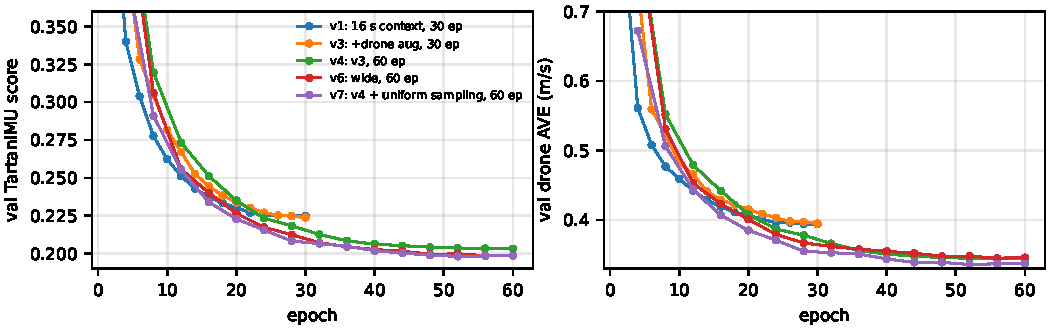
\includegraphics[width=\linewidth]{figures/val_curves.pdf}
    \caption{Val score (left) and val drone AVE (right) during training of the main development runs.}
    \label{fig:curves}
\end{figure}

\subsection{Test-Set Results}
Table~\ref{tab:overall_results} and Table~\ref{tab:platform_results} give the official numbers of the final model
(submission md5 \texttt{fd12d4f25d7b52d44aaa4e4a14534378}). The TartanIMU Score is 0.219 against 0.538 for the
organisers' baseline. The car, handheld and quadruped AVE are 0.071, 0.053 and 0.074\,m/s; the drone AVE is
0.522\,m/s and, together with the drone ATE$_{20}$ of 1.04\,m, accounts for 64\,\% of the score. The public
leaderboard score is 0.286; the public subset is dominated by short racing-drone clips (Sec.~\ref{sec:data}), and we
measured differences of $\pm$0.01--0.02 on it between runs of the same recipe on different GPUs, so we selected our
entries by val and not by leaderboard. Per-sequence numbers are in the challenge report in the code repository.
\begin{table}[htbp]
    \centering\footnotesize
    \caption{Overall challenge performance (official scoring service, full 89-sequence test set). The TartanIMU Score is
    $0.6\,\mathrm{AVE}/0.7356 + 0.4\,\mathrm{ATE}_{20}/3.1160$, dimensionless, \emph{lower is better} (all-zero = 1.000).
    \textbf{RTE does not enter the ranking}; it is defined in the caption of Table~\ref{tab:sequence_results}.
    Baseline numbers are the organizers' published full-test values.}
    \setlength{\tabcolsep}{3.5pt}
    \begin{tabular}{lcccc}
        \toprule Method & Score $\downarrow$ & ATE$_{20}$ $\downarrow$ & AVE $\downarrow$ & RTE $\downarrow$ \\ \midrule
        TartanIMU Baseline & 0.538 & 1.261 & 0.461 & -- \\
        Ours (Hack2Publish) & 0.2190 & 0.563 & 0.180 & 0.868 \\
        \bottomrule
    \end{tabular}
    \label{tab:overall_results}
\end{table}

\begin{table}[htbp]
    \centering\footnotesize
    \caption{Performance by platform (official scoring service). RTE is defined in the caption of Table~\ref{tab:sequence_results}.}
    \begin{tabular}{lccc}
        \toprule Platform & ATE$_{20}$ $\downarrow$ & AVE $\downarrow$ & RTE $\downarrow$ \\ \midrule
        Wheeled / Car & 0.369 & 0.071 & 0.323 \\
        Handheld / Human & 0.490 & 0.053 & 0.270 \\
        Legged / Quadruped & 0.358 & 0.074 & 0.353 \\
        Aerial / Drone & 1.037 & 0.522 & 2.528 \\
        \midrule Average & 0.563 & 0.180 & 0.868 \\
        \bottomrule
    \end{tabular}
    \label{tab:platform_results}
\end{table}


\subsection{Where the Error Lives}
\label{sec:data}
Fig.~\ref{fig:scatter} plots the per-trajectory val error of the final recipe against the mean speed of the
trajectory. Car, quadruped and handheld sequences sit at 0.07--0.13\,m/s regardless of speed. The drone sequences
split into two groups by source. Drone-B (246 training trajectories, 3.4\,h) sits at 0.15--0.4\,m/s and is more
accurate at 3--4\,m/s than when hovering: for the slowest sequences the error equals the standard deviation of the
ground-truth velocity itself, which is what predicting the mean gives, and hover drift below 0.2\,m/s is not visible
in the IMU. Drone-A, the racing drone (43 training trajectories, about 30\,min), sits at 0.45--1.0\,m/s at every
speed, and no amount of oversampling, augmentation, capacity or training length moved it.

We found two reasons in the data. First, the frame conventions of drone-B differ from everything else: its gyroscope
$z$ axis is inverted with respect to the body frame of its quaternion and velocity (ground-truth yaw rate $=
-\omega_z$, $R^2 = 0.97$), and its accelerometer dynamics are not a rotation of the ground-truth specific force under
any axis relabelling (the $R^2$ at 2\,Hz is negative; an unconstrained $3\times3$ fit has axis gains between 0.6 and
2.1). The other three platforms and drone-A have identity conventions with $R^2$ 0.97--0.99. The network learns
drone-B anyway because the source is easy to recognise from the signal (its high-frequency accelerometer content is
ten times lower), but what it learns there does not transfer to drone-A. Second, every fast flight of drone-A is
recorded twice, by a level IMU and by one pitched about $45^\circ$. Cross-correlating $|\omega|$ with the angular rate
derived from the quaternions shows that the two IMU streams are offset from the ground truth by different amounts,
about $-10$\,ms for one and $-40$ to $-70$\,ms for the other. After aligning the two recordings in time and fitting
the best rotation between them, their velocity labels still disagree by 0.15--0.9\,m/s, i.e.\ about $5^\circ$ of
mounting inconsistency at 4--7\,m/s. A model that sees only one IMU cannot do better than this disagreement, and
about a quarter of the test drone trajectories are of this type. Several quadruped trajectories also have offsets of
40--150\,ms, which cost little at their speeds.

\begin{figure}[t]
    \centering
    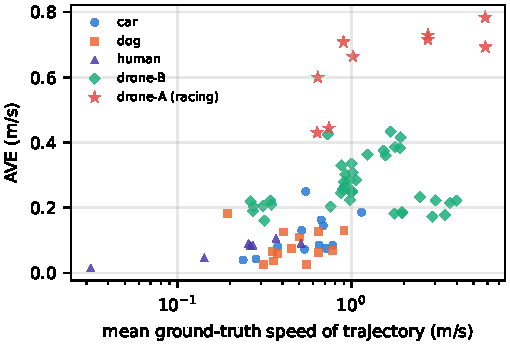
\includegraphics[width=0.9\linewidth]{figures/val_scatter.pdf}
    \caption{Per-trajectory val AVE of the final recipe against mean ground-truth speed. The racing-drone source is an
    outlier at every speed; the slowest drone-B sequences sit at the floor set by hover drift.}
    \label{fig:scatter}
\end{figure}

\section{Discussion}
Is one model enough? For the observable part of the problem, yes: a single 3.9\,M-parameter network with no platform
input reaches 0.05--0.07\,m/s on three platforms and about 0.27\,m/s on ordinary drone flight, it recognises the
embodiment on its own, and every change that helped one platform helped the others; we never found a reason to add a
platform-specific component. The bottleneck is not the model but the data. The largest residual error comes from one
source whose labels are internally inconsistent at the level of tens of milliseconds and a few degrees, and the second
largest from a motion regime the sensor cannot observe. Per hour of data, the slow and clean drone-B recordings taught
the network far more than the fast and noisy racing-drone recordings.

What transfers beyond this benchmark is the recipe rather than the weights: trajectory context, metric-shaped
sampling and physics-exact augmentation depend on no particular IMU or vehicle. What does not transfer is anything the
network has learned about a source's axis convention or timing offset -- and in a platform-blind test set whose
sources are recognisable from the signal, that knowledge is rewarded. Two things follow for benchmark design: the
synchronisation and frame conventions of every source should be verified and documented, and a held-out platform or
a causal evaluation track would measure generalisation more directly than a platform-blind split.

\section{Limitations}
The method is offline; it uses future samples of the same trajectory and would need a different design for online
use. All conclusions about the drone data are measured on the released training and validation files; we have not
inspected the test ground truth. The final model combines two changes (uniform sampling and the wider trunk) that
were validated separately but not jointly on val. Seeds were not varied, and the leaderboard noise we report is
measured from two runs only.

\section{Conclusion}
A context network over whole trajectories, trained with a sampler that mirrors the metric and with augmentation that
respects the sensor physics, gives a single inertial velocity estimator that works across four embodiments with one
set of weights and no post-processing, reaching 0.219 on the TartanIMU test set. The remaining error is dominated by
one drone source whose ground truth disagrees with itself; closing it needs better data, or models that estimate
synchronisation and mounting explicitly and with an uncertainty. Weights, inference code and training code are
available at \hfrepo{} and \ghrepo.

\section*{Acknowledgment}
We thank the CMU AirLab team for the dataset, the scorer and the scoring service.

\begin{thebibliography}{99}
\bibitem{tartanimu} S.~Zhao, S.~Zhou, R.~Blanchard, Y.~Qiu, W.~Wang, and S.~Scherer, ``Tartan IMU: A light foundation
model for inertial positioning in robotics,'' in \emph{Proc.\ IEEE/CVF CVPR}, 2025, pp.~22520--22529.
\bibitem{ronin} S.~Herath, H.~Yan, and Y.~Furukawa, ``RoNIN: Robust neural inertial navigation in the wild: Benchmark,
evaluations, \& new methods,'' in \emph{Proc.\ IEEE ICRA}, 2020, pp.~3146--3152.
\bibitem{tlio} W.~Liu, D.~Caruso, E.~Ilg, J.~Dong, A.~I. Mourikis, K.~Daniilidis, V.~Kumar, and J.~Engel, ``TLIO: Tight
learned inertial odometry,'' \emph{IEEE Robot.\ Autom.\ Lett.}, vol.~5, no.~4, pp.~5653--5660, 2020.
\bibitem{ionet} C.~Chen, X.~Lu, A.~Markham, and N.~Trigoni, ``IONet: Learning to cure the curse of drift in inertial
odometry,'' in \emph{Proc.\ AAAI}, 2018.
\bibitem{ridi} H.~Yan, Q.~Shan, and Y.~Furukawa, ``RIDI: Robust IMU double integration,'' in \emph{Proc.\ ECCV}, 2018.
\bibitem{airimu} Y.~Qiu, C.~Wang, C.~Xu, Y.~Chen, X.~Zhou, Y.~Xia, and S.~Scherer, ``AirIMU: Learning uncertainty
propagation for inertial odometry,'' \emph{arXiv:2310.04874}, 2023.
\bibitem{airio} Y.~Qiu, C.~Wang, C.~Xu, Y.~Chen, X.~Zhou, Y.~Xia, and S.~Scherer, ``AirIO: Learning inertial odometry
with enhanced IMU feature observability,'' \emph{arXiv:2501.15659}, 2025.
\bibitem{titterton} D.~H. Titterton and J.~L. Weston, \emph{Strapdown Inertial Navigation Technology}, 2nd ed.
IET, 2004.
\bibitem{sturm2012rgbd} J.~Sturm, N.~Engelhard, F.~Endres, W.~Burgard, and D.~Cremers, ``A benchmark for the
evaluation of RGB-D SLAM systems,'' in \emph{Proc.\ IEEE/RSJ IROS}, 2012, pp.~573--580.
\end{thebibliography}

\end{document}
